\documentclass[a4paper, 14pt]{article}
\usepackage{float}
\usepackage{geometry}
\usepackage{graphicx}
\usepackage[utf8]{inputenc}
\usepackage{setspace}
\usepackage{lmodern}
\usepackage[hidelinks]{hyperref}

\linespread{1.5}
\newcommand\tab[1][1cm]{\hspace*{#1}}
\geometry{left=20mm,right=20mm,top=20mm,bottom=20mm}
\begin{document}
\fontfamily{ptm}\selectfont
{
\pagenumbering{arabic}
\begin{center}	
\textbf{\fontsize{18}{2} \selectfont POST MERGER ANALYSIS OF CUSTOMER SATISFACTION AND LOYALTY - A STUDY ON RECENT MERGER OF ASSOCIATE BANKS OF SBI WITH ITSELF}\\
\tab \\
\textbf{\fontsize{14}{2} \selectfont REVIEW 3 - REPORT}\\
\tab \\
\textbf{\fontsize{14}{2} \selectfont \emph{Submitted by}}\\
\tab \\
\tab \\
{\fontsize{16}{2} \selectfont
\textbf{ADHITHYAN V}}\\
{\fontsize{16}{2} \selectfont \textbf{(2016201002)}}\\

\textbf{\fontsize{16}{2} \selectfont MASTER OF BUSINESS ADMINISTRATION}\\
\begin{figure}[H]
\centering

\includegraphics[scale=0.5]{anna_univ_logo.jpg}
\end{figure}
\tab \\
\textbf{\fontsize{14}{2} \selectfont COLLEGE OF ENGINEERING, GUINDY}\\
\tab \\
\textbf{\fontsize{16}{2} \selectfont ANNA UNIVERSITY : CHENNAI 600 025}\\
\tab \\
{\fontsize{14}{2} \selectfont APRIL 2018}\\
\end{center}
\newpage
\section*{DATA COLLECTION}
Data was collected in 2 modes \textbf{online} mode using \textbf{Google Forms} and \textbf{offline mode} in which some part of data was collected from erstwhile SBT pollachi branch and SBH Thiruvanmiyur branch. For online mode data collection twitter was used as medium to communicate with people. Those who have mentioned SBH, SBT, SBBJ, SBP and SBM were identified from their tweets and they were contacted to obtain response.
\section*{ANALYSIS}
\subsection*{No of data}
 A total of \textbf{101} responses were obtained using Google forms and some of the data was collected in the bank premises in Chennai and Pollachi.
\subsection*{Demographics}
\par Out of 101 responses
\begin{itemize}
\item 17 were Female (16.8 \%)
\item 84 were Male (83.2 \%)
\end{itemize}
\begin{figure}[H]
\centering
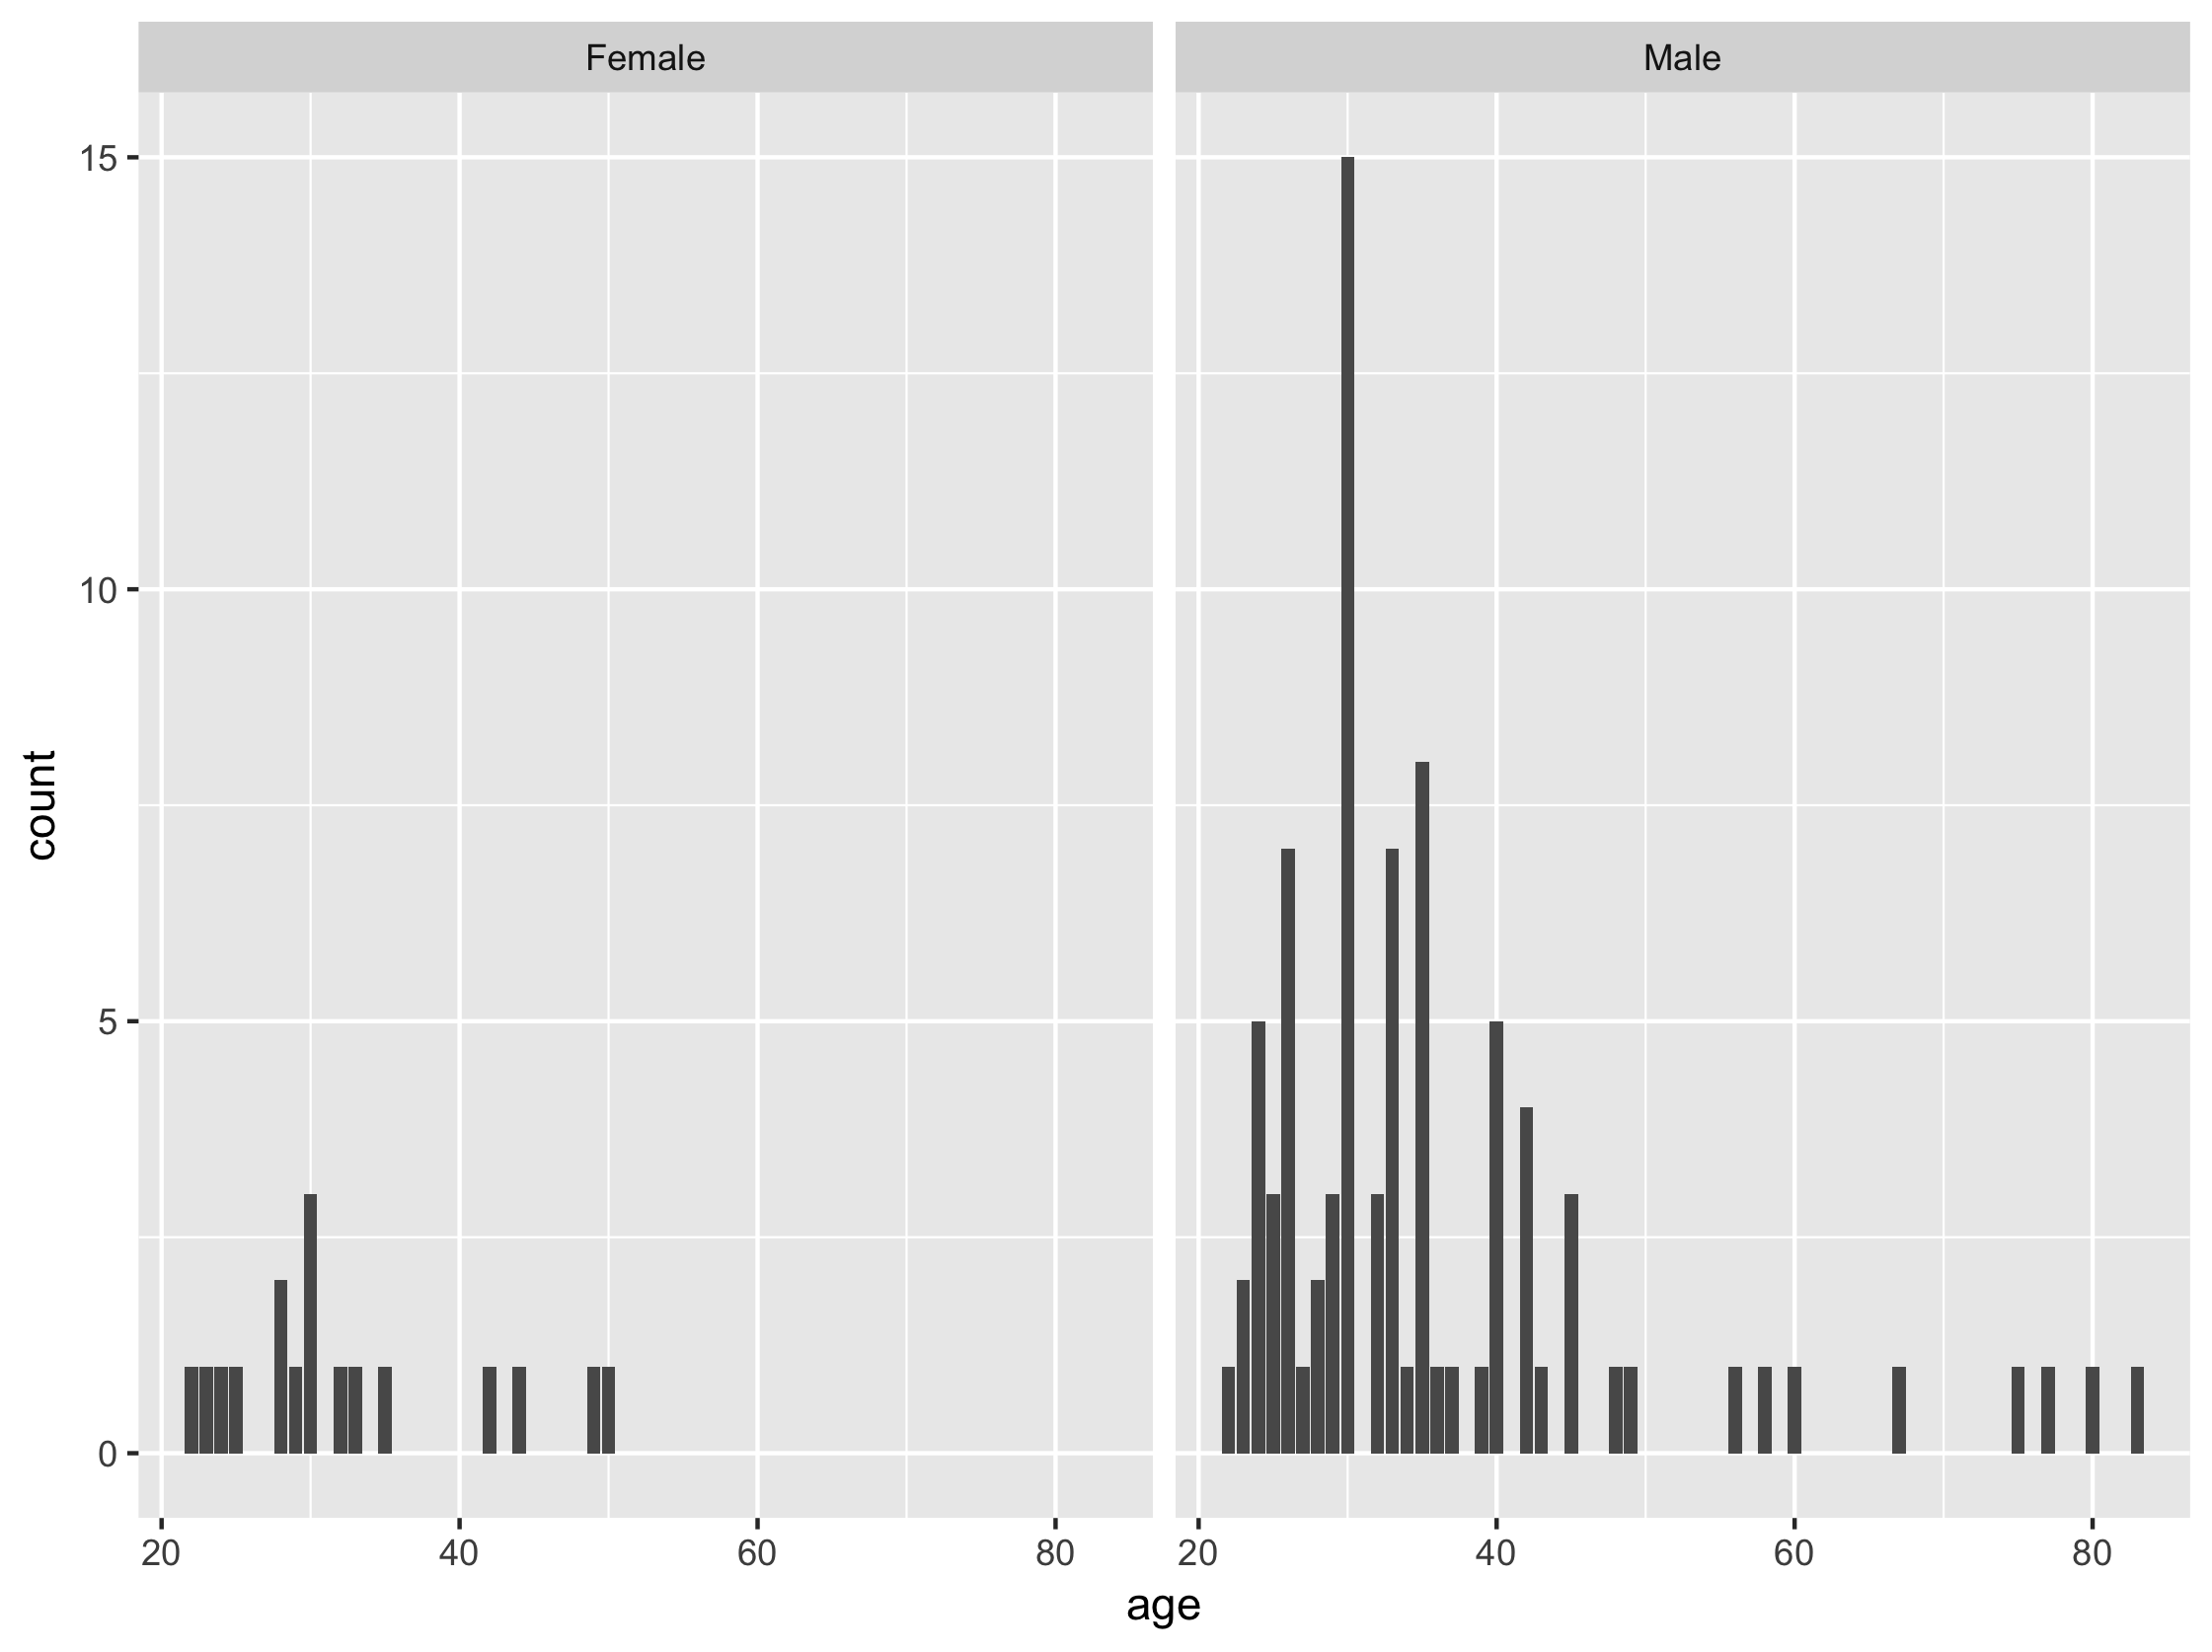
\includegraphics[scale=0.2]{age_distribution.png}
\caption{Age distribution of respondents}
\end{figure}
\subsection*{Cronbach's alpha}
\begin{center}
\begin{tabular}{|c|c|c|}
\hline
\textbf{Scale name} & \textbf{Cronbach $\alpha$} & \textbf{No of items}\\
\hline
Psychological Contract Violation & \textbf{0.89} & 8\\
Service Performance & \textbf{0.712} & 10\\
Customer Satisfaction & \textbf{0.96} & 4\\
Customer Loyalty & \textbf{0.927} & 5 \\
\hline
\end{tabular}
\end{center}

\subsection*{DESCRPTIVE STATISTICS}
\begin{table}[H]
\centering
\begin{tabular}{|c|c|c|c|}
\hline
Item & \textbf{Mean} & \textbf{SD} & N \\
\hline
Customer satisfaction & 2.968 & 1.37 & 101 \\
\hline
PCV & 3.06 & 0.98 & 101 \\
\hline
Overall service & 2.80 & 1.49 & 101 \\
\hline
Service performance & 3.01 & 1.0428 & 101 \\
\hline
Loyalty & 3.07 & .368 & 101 \\
\hline
\end{tabular}
\caption{Descriptive Statistics}
\end{table}

\subsection*{HYPOTHESIS}
\begin{itemize}
\item H1 - Psychological Contract Violation has negative influence on customer satisfaction.
\item H2 - Service performance is a determinant of Overall Service
\item H3 - Overall service has a positive impact on customer satisfaction
\item H4 - Customer satisfaction has positive influence on customer loyalty.
\end{itemize}

\subsection*{Pearson Correlation}
\begin{center}
\begin{tabular}{|c|c|}
\hline
Variables & Correlation Value \\
\hline
PCV vs Customer Satisfaction & \textbf{-0.662} \\
Service Performance vs Overall Service & \textbf{-0.830} \\
Overall service vs Customer Satisfaction & \textbf{0.907} \\
Customer Satisfaction vs Customer Loyalty & \textbf{0.602} \\
\hline
\end{tabular}
\end{center}

\subsection*{MODEL SUMMARY}
\begin{figure}[H]
\centering
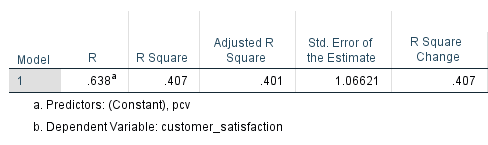
\includegraphics[scale=1]{pcv_vs_customer_satisfaction.png}
\end{figure}

\begin{figure}[H]
\centering
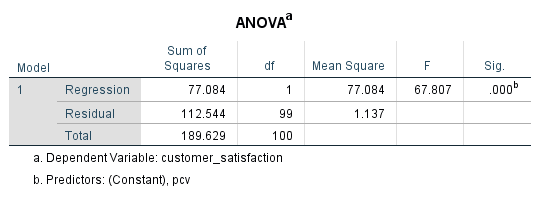
\includegraphics[scale=1]{anova_pcv_cs.png}
\caption{H1 - Psychological Contract Violation has negative influence on customer satisfaction.}
\end{figure}


\begin{figure}[H]
\centering
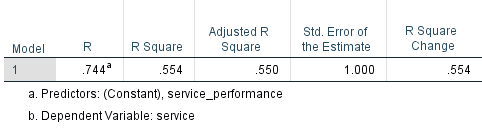
\includegraphics[scale=1]{service_performance_vs_service.png}
\end{figure}

\begin{figure}[H]
\centering
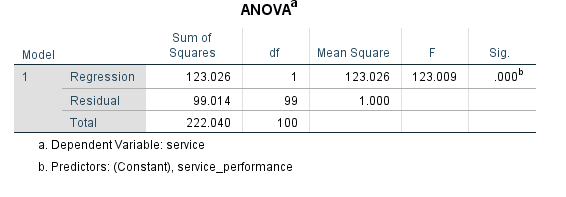
\includegraphics[scale=1]{anova_s_sp.png}
\caption{H2 - Service performance is a determinant of Overall Service}
\end{figure}


\begin{figure}[H]
\centering
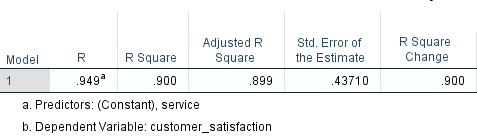
\includegraphics[scale=1]{sp_vs_cs.png}
\end{figure}

\begin{figure}[H]
\centering
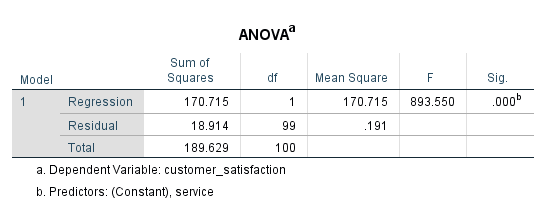
\includegraphics[scale=1]{anova_css.png}
\caption{H3 - Overall service has a positive impact on customer satisfaction}
\end{figure}

\begin{figure}[H]
\centering
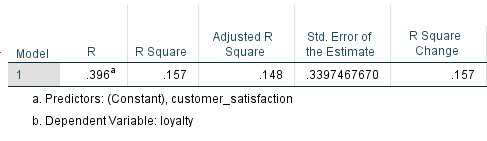
\includegraphics[scale=1]{customer_satisfaction_vs_loyalty.png}
\end{figure}

\begin{figure}[H]
\centering
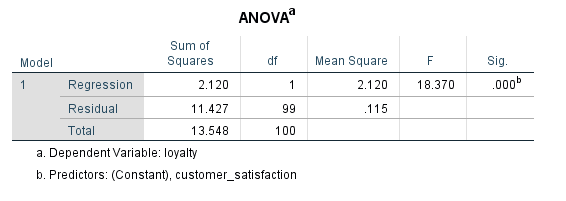
\includegraphics[scale=1]{anova_cs_lo.png}
\caption{H4 - Customer satisfaction has positive influence on customer loyalty.}
\end{figure}

\begin{table}[H]
\centering
\begin{tabular}{|c|c|c|}
\hline
Question & Mean & SD \\
\hline
\textbf{ I feel happy about the merger.} & 3.6 & 1.26 \\
\hline
\textbf{ I feel pleased about the merger} & 4.2 & 1.19 \\
\hline
\textbf{ I feel disappointed about the merger } & 2.4 & 1.1 \\
\hline
\textbf{ I feel violated about the merger} & 1.9 & 0.5 \\
\hline
\textbf{ I feel grateful about the merger} & 3.2 & 1.01 \\
\hline
\textbf{ I have difficulty in obtaining information post merger. } & 2.73 & 1.4 \\
\hline
\textbf{ I find difficult to commute.} & 2.3 & 1.47 \\
\hline    
\textbf{ I lost my personal care / identity after merger. } & 4.2 & 1.2 \\
\hline
\textbf{ Time required to avail a service.} & 3.3 & 1.3 \\
\hline
\textbf{ Effort taken to receive a service.}  & 3.5 & 1.42 \\ 
\hline
\textbf{ Employees provide consistent service.}  & 3.15 & 0.6\\  
\hline
\textbf{ Employees are willing and provide service in a timely manner.} & 3.19 & 1.244\\
\hline
\textbf{ Employees are approachable and easy to contact.} & 3.08 & 0.309\\   
\hline
\textbf{ Employees are courteous, polite and respectful.} & 4.03 & 0.8 \\
\hline
\textbf{ Employees listen and speak to me in  a language I understand.} & 2.05 & 0.994 \\
\hline
\textbf{ Employees are trustworthy, honest and believable.} & 3.05 & 0.506 \\
\hline
\textbf{ Employees make effort to understand my needs.} & 2.7 & 1 \\
\hline
\textbf{ Physical facilities and employees are neat and clean.} & 1.5 & 0.876\\
\hline
\textbf{ The overall ability of bank to satisfy my needs and wants is.} & 3.65 & 1.445 \\
\hline
\textbf{ Overall satisfaction level} & 2.85 & 2.3 \\
\hline
\textbf{ To what extent, service has met expectation ?} & 3.75 & 1.4 \\
\hline
\textbf{ Compare the current service with before merger.} & 2.3 & 1.363 \\
\hline
\textbf{ Would you recommend to a friend / relatives?} & 2.2 & 1.19 \\
\hline
\textbf{ Will you avail service continuosly ?} & 2.5 & 1.2 \\
\hline
\textbf{ Will you open account again ?} & 1.14 & 1.18 \\
\hline
\textbf{ I had a problem or negative experience after merger?} & 3.9 & 0.561 \\
\hline
\textbf{ Given an option to switch, I will switch to other banks.} & 4.43 & 1.525 \\
\hline
\end{tabular}
\end{table}



\section*{INTERPRETATION}
\begin{itemize}
\item PCV and customer satisfaction are negatively correlated (-0.662). This indicates as customer perceives more PCV, satisfaction declines. \textbf{H1 is accepted}
\item Service performance is negatively correlated with overall service (-0.830). This indicates overall service doesn't depend on service performance. \textbf{H2 is rejected}
\item Overall service has a positive correlation with customer satisfaction (0.907). As overall service increases, customer satisfaction tends to increase. 
\textbf{H3 is accepted}
\item Customer satisfaction and loyalty are postively correlated (0.602). This indicates a satisfied customer will be more loyal to the bank and spreads word of mouth.\textbf{H4 is accepted.}
\item PCV explains 40.1\% variance in customer satisfaction.
\item Service performance explains 55\% of variance in overall service.
\item Overall service explains 89.9\% of variance in customer satisfaction.
\item Customer satisfaction explains 15.7\% of variance in loyalty.
\end{itemize}
\section*{FINDINGS}
The data analyses reveal that merger of State Bank of India with its associate banks has not made much negative impact on its customers. Psychological Contract Breach, Customer Satisfaction and Loyalty is medium while service performance is low.

PCV is very medium. Majority of people claimed that they lost their identities after merger. The number people who found difficult to commute was average and the difficulty in getting information was also average.

Customers feel that service performance before and after merger remains more or less same. They didn't see any drastic improvement in service. SBI continues to be SBI one of the respondent quoted. Majority of the customers felt that employees were rude. They were not courteous. Most of the respondents felt that service had met expectation while the after merger service performance was not ideal.

Now that all the associate banks have merged with SBI, the customer base of the bank has become huge. And so, number of customers visiting the bank has also increased. Customers who previously had to travel long to reach any of the associate bank in which he had account ,can now get his job done at any of the nearby branches of the SBI. For example in pollachi before merger there was SBI and SBT. SBI will always be crowdy, since it's located close to bus stand. After merger considerable crowd has decreased and they go to SBT where there is less crowd. It can be inferred that customer satisfaction is also medium.

Loyalty is also medium indicating that people doesn't become mascots for SBI. Many people claimed that private banks offer far better services than SBI like priority banking etc. They mentioned that some had no other choice other than opening with SBI due to circumstances. If now they are offered an option to switch they will definitely switch to other banks as evident from the descriptive statistics table.


\section*{CONCLUSION}
\par Though merger is beneficial to management in terms of financial perspective and synergies, merger often brings a lot of pain to customer. In our case many branches were shut down, customers lost identities etc. So merger should be planned with customer in mind to ensure smooth functioning and service.
\section*{FUTURE RESEARCH DIRECTIONS}
\par During response collection it was found that, many of the people preferred private banks over SBI/PSU banks. So a study can be conducted to know the areas in which private banks excel and it can be used to improve the service of PSU banks.
}
\end{document}